\documentclass[12pt,a4paper]{article}
\usepackage{cmap} % Makes the PDF copiable. See http://tex.stackexchange.com/a/64198/25761
\usepackage[T1]{fontenc}
\usepackage[brazil]{babel}
\usepackage[utf8]{inputenc}
\usepackage{amsmath}
\usepackage{amsfonts}
\usepackage{amssymb}
\usepackage{amsthm}
\usepackage{textcomp} % \degree
\usepackage{gensymb} % \degree
\usepackage[usenames,svgnames,dvipsnames]{xcolor}
\usepackage{hyperref}
\usepackage{multicol}
\usepackage{graphicx}
\usepackage[margin=2cm]{geometry}
\usepackage{icomma} % vírgulas como pontuação vs ponto decimal
\hypersetup{
    colorlinks = true,
    allcolors = {blue}
}

\newcommand{\fixme}{{\color{red}(...)}}
\newcommand*\sen{\operatorname{sen}}
\newcommand*\tg{\operatorname{tg}}
\newcommand*\arctg{\operatorname{arctg}}
\newcommand*\R{\mathbb{R}}
\newcommand*\diff{\mathop{}\!\mathrm{d}}

\newcommand{\IconPc}{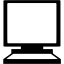
\includegraphics[width=1em]{computer.png}}
\newcommand{\IconCalc}{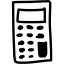
\includegraphics[width=1em]{calculator.png}}
\newcommand{\IconThink}{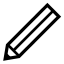
\includegraphics[width=1em]{pencil.png}}
\newcommand{\IconCheck}{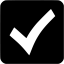
\includegraphics[width=1em]{checkmark.png}}
\newcommand{\IconConcept}{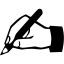
\includegraphics[width=1em]{edit.png}}

\newlength{\SmileysLength}
\setlength{\SmileysLength}{\labelwidth}\addtolength{\SmileysLength}{\labelsep}

\newcommand{\calc}{\hspace*{-\SmileysLength}\makebox[0pt][r]{\IconCalc}%
   \hspace*{\SmileysLength}}
\newcommand{\software}{\hspace*{-\SmileysLength}\makebox[0pt][r]{\IconPc}%
   \hspace*{\SmileysLength}}
\newcommand{\teoria}{\hspace*{-\SmileysLength}\makebox[0pt][r]{\IconThink}%
   \hspace*{\SmileysLength}}
\newcommand{\conceito}{\hspace*{-\SmileysLength}\makebox[0pt][r]{\IconCheck}%
   \hspace*{\SmileysLength}}
\newcommand{\concept}{\hspace*{-\SmileysLength}\makebox[0pt][r]{\IconCheck}%
   \hspace*{\SmileysLength}}

\newcommand*\tipo{Lista de Exercícios - Equações Diferenciais}
%\newcommand*\turma{...}
\newcommand*\disciplina{ANN0001/CAN0001}
\newcommand*\eu{Helder G. G. de Lima}
\newcommand*\data{\today}

\author{\eu}
\title{\tipo}
\date{\data}

\begin{document}

\begin{center}

\includegraphics[width=9.0cm]{marca} \\
\textbf{\tipo} \\
Prof. \eu\footnote{
Este é um material de acesso livre distribuído sob os termos da licença \href{https://creativecommons.org/licenses/by-sa/4.0/deed.pt_BR}{Creative Commons BY-SA 4.0}.}
\end{center}

%\section*{Legenda}
%\begin{multicols}{4}
%\begin{itemize}
%\item[] \hspace*{\SmileysLength} \calc \hspace*{-\SmileysLength} Cálculos
%\item[] \hspace*{\SmileysLength} \conceito \hspace*{-\SmileysLength} Conceitos
%\item[] \hspace*{\SmileysLength} \teoria \hspace*{-\SmileysLength} Teoria
%\item[] \hspace*{\SmileysLength} \software \hspace*{-\SmileysLength} Software
%\end{itemize}
%\end{multicols}

\section*{Questões}

\begin{enumerate}
\item A seguir são dados vários problemas de valor inicial, juntamente com a sua solução exata. Use cada um dos métodos estudados para estimar os valores de $y(x)$ conforme $x$ percorre o intervalo $[a,b]$, usando um passo $h$ do tamanho indicado. Faça uma tabela com os valores exatos ($y(x_i)$) e aproximados ($y_i$), em cada ponto $x_i$. Compare esses resultados para determinar o maior erro absoluto (em módulo) cometido nos pontos considerados.
\begin{enumerate}
\item $\begin{cases}
y^\prime = x-\frac{y}{x} \\
y(1) = -1
\end{cases}$
Utilize $h = 0,25$ e $[a,b] = [1, 2]$. A solução exata é $y = \frac{x^3 - 4}{3x}$.
\item $\begin{cases}
y^\prime = x+y \\
y(0) = 0
\end{cases}$
Utilize $h = 0,4$ e $[a,b] = [0, 2]$. A solução exata é $y = e^x - x - 1$.
\item $\begin{cases}
y^\prime = \sen(x) - \frac{x}{2} \\
y(0) = -1
\end{cases}$
Utilize $h = \frac{1}{2}$ e $[a,b] = [0,2]$. A solução exata é $y = \frac{-x^2}{4} - \cos(x)$.
\item $\begin{cases}
y^\prime = y \cos(x) \\
y(0) = 1
\end{cases}$
Utilize $h = \frac{1}{3}$ e $[a,b] = [0,2]$. A solução exata é $y = e^{\sen(x)}$.
\end{enumerate}

\item Resolva os problemas de valor inicial a seguir, utilizando o método de Euler com passos $h = 0.25$ e $h=0.125$, para obter aproximações para $y_1(1)$ e $y_2(1)$.
\begin{multicols}{2}
\begin{enumerate}
\item $\begin{cases}
y_1^\prime(t) &= 4y_2(t)\\
y_2^\prime(t) &= -4y_1(t)\\
y_1(0) &= 0\\
y_2(0) &= 2
\end{cases}$

\item $\begin{cases}
y_1^\prime(t) &= y_1(t) y_2(t)\\
y_2^\prime(t) &= y_1(t)+y_2(t)\\
y_1(0) &= 7\\
y_2(0) &= -1
\end{cases}$
\end{enumerate}
\end{multicols}

\item Aplique os métodos de Euler explícito e implícito, e os métodos de Runge-Kutta de ordem 2 e 4 para obter soluções aproximadas do problema de valor inicial
\[
\begin{cases}
y^\prime(t) = 6t - 3y(t) \\
y(0) = 1.
\end{cases}\]
Utilize passos de tamanho $h = 0,2$ ao longo do intervalo $[a, b] = [0, 1]$. Faça um gráfico para comparar as soluções obtidas e a solução exata, que é $y(t) = \frac{1}{3} (6 t - 2 + 5 e^{-3 t})$.
\end{enumerate}


\newpage
\section*{Algumas respostas}

\begin{enumerate}
\item \begin{enumerate}
\item Neste PVI, tem-se $f(x, y) = x - \frac{y}{x}$ e será usado $h = 0,25$.
\begin{itemize}
\item \textbf{Método de Euler explícito}: A aproximação $y_{i + 1}$, para $0 \leq i \leq 3$, é dada por
\[
y_{i + 1}
= y_{i} + 0,25 \cdot \left( x_i - \frac{y_i}{x_i} \right).
\]
Disto resulta que os valores obtidos a cada passo são os seguintes:

\medskip
\begin{center}
\begin{tabular}{ccrrr}
\hline
$i$ & $x_i$ & $y_i$ & $y_{exato}(x_i)$ & $\varepsilon_i = y_i-y_{exato}(x_i)$ \\ \hline
$0$ & $1,0000$ & $-1,0000$ & $-1,0000$ & $0,0000$ \\
$1$ & $1,2500$ & $-0,5000$ & $-0,5458$ & $0,0458$ \\
$2$ & $1,5000$ & $-0,0875$ & $-0,1389$ & $0,0514$ \\
$3$ & $1,7500$ & $ 0,3021$ & $ 0,2589$ & $0,0432$ \\
$4$ & $2,0000$ & $ 0,6965$ & $ 0,6667$ & $0,0298$ \\
\hline
\end{tabular}
\end{center}
\medskip
O maior erro absoluto em módulo foi $|\varepsilon_2| = 0,0514$, em $x_2 = 1,5$.

\item \textbf{Método de Euler implícito}: Neste caso, $y_{i + 1}$ é dado implicitamente por
\[
y_{i + 1}
= y_{i} + 0,25 \cdot \left( x_{i + 1} - \frac{y_{i + 1}}{x_{i + 1}} \right),
\quad 0 \leq i \leq 3.
\]
Resolvendo a equação, resulta que $y_{i + 1}$ é dado por:
\[
y_{i + 1}
= \frac{x_{i + 1} \left(y_{i} + 0,25 x_{i + 1}\right)}{ x_{i + 1} + 0,25 }.
\]
Disto resulta que os valores obtidos a cada passo são os seguintes:

\medskip
\begin{center}
\begin{tabular}{ccrrr}
\hline
$i$ & $x_i$ & $y_i$ & $y_{exato}(x_i)$ & $\varepsilon_i = y_i-y_{exato}(x_i)$ \\ \hline
$0$ & $1,0000$ & $-1,0000$ & $-1,0000$ & $ 0,0000$ \\
$1$ & $1,2500$ & $-0,5729$ & $-0,5458$ & $-0,0271$ \\
$2$ & $1,5000$ & $-0,1696$ & $-0,1389$ & $-0,0307$ \\
$3$ & $1,7500$ & $ 0,2344$ & $ 0,2589$ & $-0,0245$ \\
$4$ & $2,0000$ & $ 0,6528$ & $ 0,6667$ & $-0,0139$ \\
\hline
\end{tabular}
\end{center}
\medskip
O maior erro absoluto em módulo foi $|\varepsilon_2| = 0,0307$, em $x_2 = 1,5$.


\item \textbf{Método de Runge-Kutta de 2ª ordem}: Considerando
$k_1 = f(x_i, y_i)$,
$k_2 = f(x_i + h, y_i + k_1 h)$, e
$y_{i+1} = y_i + \frac{h}{2} (k_1 + k_2)$, obtém-se:
\medskip
\begin{center}
    \begin{tabular}{crrrrrr}
    \hline
      $i$ & $x_i$  & $y_i$ & $k_1$ & $k_2$ & $y_{exato}(x_i)$
      & $\varepsilon_i = y_i-y_{exato}(x_i)$ \\ \hline
    $0$ & $1,0000$ & $-1,0000$ & $2,0000$ & $1,6500$ & $-1,0000$ & $0,0000$ \\
    $1$ & $1,2500$ & $-0,5438$ & $1,6850$ & $1,5817$ & $-0,5458$ & $0,0020$ \\
    $2$ & $1,5000$ & $-0,1355$ & $1,5903$ & $1,6002$ & $-0,1389$ & $0,0034$ \\
    $3$ & $1,7500$ & $ 0,2633$ & $1,5995$ & $1,6684$ & $ 0,2589$ & $0,0044$ \\
    $4$ & $2,0000$ & $ 0,6718$ & $1,6641$ & $1,7665$ & $ 0,6667$ & $0,0051$ \\
    \hline
    \end{tabular}
\end{center}
\medskip
O maior erro absoluto em módulo foi $|\varepsilon_4| = 0,0051$, em $x_4 = 2$.

\item \textbf{Método de Runge-Kutta de 4ª ordem}: Considerando
$k_1 = f(x_i, y_i)$,
$k_2 = f(x_i + \frac{h}{2}, y_i + k_1 \frac{h}{2})$,
$k_3 = f(x_i + \frac{h}{2}, y_i + k_2 \frac{h}{2})$,
$k_4 = f(x_i +       h    , y_i + k_3 h)$, e
$y_{i+1} = y_i + \frac{h}{6} (k_1 + 2k_2 + 2k_3 + k_4)$, tem-se:
\begin{center}
   \begin{footnotesize}
      \begin{tabular}{crrrrrrrr}
      \hline
        $i$ & $x_i$  & $y_i$ & $k_1$ & $k_2$ & $k_3$ & $k_4$ & $y_{exato}(x_i)$
        & $y_i-y_{exato}(x_i)$ \\ \hline
      $0$ & $1,0000$ & $-1,0000$ & $2,0000$ & $1,7917$ & $1,8148$ & $1,6870$ & $-1,0000$ & $0,0000$ \\
      $1$ & $1,2500$ & $-0,5458$ & $1,6866$ & $1,6186$ & $1,6248$ & $1,5931$ & $-0,5458$ & $0,0000$ \\
      $2$ & $1,5000$ & $-0,1389$ & $1,5926$ & $1,5880$ & $1,5883$ & $1,6025$ & $-0,1389$ & $0,0000$ \\
      $3$ & $1,7500$ & $ 0,2589$ & $1,6021$ & $1,6301$ & $1,6282$ & $1,6670$ & $ 0,2589$ & $0,0000$ \\
      $4$ & $2,0000$ & $ 0,6667$ & $1,6667$ & $1,7132$ & $1,7105$ & $1,7636$ & $ 0,6667$ & $0,0000$ \\
      \hline
      \end{tabular}
   \end{footnotesize}
\end{center}
Ao arredondar os resultados exatos e as aproximações com quatro dígitos após a vírgula, o erro absoluto é zero em todos os pontos considerados.

\end{itemize}
\item Neste PVI, tem-se $f(x, y) = x + y$ e será usado $h = 0,4$.
\begin{itemize}
\item \textbf{Método de Euler explícito}: A aproximação $y_{i + 1}$, para $0 \leq i \leq 4$, é dada por
\[
y_{i + 1}
= y_{i} + 0,4 \cdot \left( x_i + y_i \right)
= 0,4 x_i + 1,4 y_{i}.
\]
Disto resulta que os valores obtidos a cada passo são os seguintes:

\medskip
\begin{center}
\begin{tabular}{ccrrr}
\hline
$i$ & $x_i$ & $y_i$ & $y_{exato}(x_i)$ & $\varepsilon_i = y_i-y_{exato}(x_i)$ \\ \hline
$0$ & $0,0000$ & $0,0000$ & $0,0000$ & $ 0,0000$ \\
$1$ & $0,4000$ & $0,0000$ & $0,0918$ & $-0,0918$ \\
$2$ & $0,8000$ & $0,1600$ & $0,4255$ & $-0,2655$ \\
$3$ & $1,2000$ & $0,5440$ & $1,1201$ & $-0,5761$ \\
$4$ & $1,6000$ & $1,2416$ & $2,3530$ & $-1,1114$ \\
$5$ & $2,0000$ & $2,3782$ & $4,3891$ & $-2,0109$ \\
\hline
\end{tabular}
\end{center}
\medskip
O maior erro absoluto em módulo foi $|\varepsilon_5| = 2,0109$, em $x_5 = 2$.

\item \textbf{Método de Euler implícito}: Neste caso, $y_{i + 1}$ é dado implicitamente por
\[
y_{i + 1}
= y_{i} + 0,4 \cdot \left( x_{i + 1} + y_{i + 1} \right),
\quad 0 \leq i \leq 4.
\]
Resolvendo a equação, resulta que $y_{i + 1}$ é dado por:
\[
y_{i + 1}
= \frac{y_{i} + 0,4 x_{i + 1}}{0,6}.
\]
Disto resulta que os valores obtidos a cada passo são os seguintes:

\medskip
\begin{center}
\begin{tabular}{ccrrr}
\hline
$i$ & $x_i$ & $y_i$ & $y_{exato}(x_i)$ & $\varepsilon_i = y_i-y_{exato}(x_i)$ \\ \hline
$0$ & $0,0000$ & $0,0000$ & $0,0000$ & $0,0000$ \\
$1$ & $0,4000$ & $0,2667$ & $0,0918$ & $0,1749$ \\
$2$ & $0,8000$ & $0,9778$ & $0,4255$ & $0,5523$ \\
$3$ & $1,2000$ & $2,4297$ & $1,1201$ & $1,3096$ \\
$4$ & $1,6000$ & $2,4297$ & $2,3530$ & $2,7632$ \\
$5$ & $2,0000$ & $9,8603$ & $4,3891$ & $5,4712$ \\
\hline
\end{tabular}
\end{center}
\medskip
O maior erro absoluto em módulo foi $|\varepsilon_5| = 5,4712$, em $x_5 = 2$.

\item \textbf{Método de Runge-Kutta de 2ª ordem}: Considerando
$k_1 = f(x_i, y_i)$,
$k_2 = f(x_i + h, y_i + k_1 h)$, e
$y_{i+1} = y_i + \frac{h}{2} (k_1 + k_2)$, obtém-se:
\medskip
\begin{center}
    \begin{tabular}{crrrrrr}
    \hline
      $i$ & $x_i$  & $y_i$ & $k_1$ & $k_2$ & $y_{exato}(x_i)$
      & $\varepsilon_i = y_i-y_{exato}(x_i)$ \\ \hline
    $0$ & $0,0000$ & $0,0000$ & $0,0000$ & $0,4000$ & $0,0000$ & $ 0,0000$ \\
    $1$ & $0,4000$ & $0,0800$ & $0,4800$ & $1,0720$ & $0,0918$ & $-0,0118$ \\
    $2$ & $0,8000$ & $0,3904$ & $1,1904$ & $2,0666$ & $0,4255$ & $-0,0351$ \\
    $3$ & $1,2000$ & $1,0418$ & $2,2418$ & $3,5385$ & $1,1201$ & $-0,0783$ \\
    $4$ & $1,6000$ & $2,1979$ & $3,7979$ & $5,7171$ & $2,3530$ & $-0,1551$ \\
    $5$ & $2,0000$ & $4,1009$ & $6,1009$ & $8,9413$ & $4,3891$ & $-0,2882$ \\
    \hline
    \end{tabular}
\end{center}
\medskip
O maior erro absoluto em módulo foi $|\varepsilon_5| = 0,2882$, em $x_5 = 2$.

\item \textbf{Método de Runge-Kutta de 4ª ordem}: Considerando
$k_1 = f(x_i, y_i)$,
$k_2 = f(x_i + \frac{h}{2}, y_i + k_1 \frac{h}{2})$,
$k_3 = f(x_i + \frac{h}{2}, y_i + k_2 \frac{h}{2})$,
$k_4 = f(x_i +       h    , y_i + k_3 h)$, e
$y_{i+1} = y_i + \frac{h}{6} (k_1 + 2k_2 + 2k_3 + k_4)$, tem-se:
\begin{center}
   \begin{footnotesize}
      \begin{tabular}{crrrrrrrr}
      \hline
        $i$ & $x_i$  & $y_i$ & $k_1$ & $k_2$ & $k_3$ & $k_4$ & $y_{exato}(x_i)$
        & $y_i-y_{exato}(x_i)$ \\ \hline
      $0$ & $0,0000$ & $0,0000$ & $0,0000$ & $0,2000$ & $0,2400$ & $ 0,4960$ & $0,0000$ & $ 0,0000$ \\
      $1$ & $0,4000$ & $0,0917$ & $0,4917$ & $0,7900$ & $0,8497$ & $ 1,2316$ & $0,0918$ & $-0,0001$ \\
      $2$ & $0,8000$ & $0,4252$ & $1,2252$ & $1,6702$ & $1,7592$ & $ 2,3289$ & $0,4255$ & $-0,0003$ \\
      $3$ & $1,2000$ & $1,1194$ & $2,3194$ & $2,9833$ & $3,1161$ & $ 3,9658$ & $1,1201$ & $-0,0007$ \\
      $4$ & $1,6000$ & $2,3517$ & $3,9517$ & $4,9420$ & $5,1401$ & $ 6,4077$ & $2,3530$ & $-0,0013$ \\
      $5$ & $2,0000$ & $4,3866$ & $6,3866$ & $7,8639$ & $8,1594$ & $10,0504$ & $4,3891$ & $-0,0025$ \\
      \hline
      \end{tabular}
   \end{footnotesize}
\end{center}
O maior erro absoluto em módulo foi $|\varepsilon_5| = 0,0025$, em $x_5 = 2$.

\end{itemize}
\item Neste PVI, tem-se $f(x, y) = \sen(x) - \frac{x}{2}$ e será usado $h = 0,5$.
\begin{itemize}
\item \textbf{Método de Euler explícito}: A aproximação $y_{i + 1}$, para $0 \leq i \leq 3$, é dada por
\[
y_{i + 1}
= y_{i} + 0,5 \cdot \left( \sen(x_i) - \frac{x_i}{2} \right).
\]
Disto resulta que os valores obtidos a cada passo são os seguintes:

\medskip
\begin{center}
\begin{tabular}{ccrrr}
\hline
$i$ & $x_i$ & $y_i$ & $y_{exato}(x_i)$ & $\varepsilon_i = y_i-y_{exato}(x_i)$ \\ \hline
$0$ & $0,0000$ & $-1,0000$ & $-1,0000$ & $ 0,0000$ \\
$1$ & $0,5000$ & $-1,0000$ & $-0,9401$ & $-0,0599$ \\
$2$ & $1,0000$ & $-0,8853$ & $-0,7903$ & $-0,0950$ \\
$3$ & $1,5000$ & $-0,7146$ & $-0,6332$ & $-0,0814$ \\
$4$ & $2,0000$ & $-0,5909$ & $-0,5839$ & $-0,0070$ \\
\hline
\end{tabular}
\end{center}
\medskip
O maior erro absoluto em módulo foi $|\varepsilon_2| = 0,0950$, em $x_2 = 1$.

\item \textbf{Método de Euler implícito}: Neste caso, $y_{i + 1}$ é dado por
\[
y_{i + 1}
= y_{i} + 0,5 \cdot \left( \sen(x_{i + 1}) - \frac{x_{i + 1}}{2} \right),
\quad 0 \leq i \leq 3.
\]
Disto resulta que os valores obtidos a cada passo são os seguintes:

\medskip
\begin{center}
\begin{tabular}{ccrrr}
\hline
$i$ & $x_i$ & $y_i$ & $y_{exato}(x_i)$ & $\varepsilon_i = y_i-y_{exato}(x_i)$ \\ \hline
$0$ & $0,0000$ & $-1,0000$ & $-1,0000$ & $ 0,0000$ \\
$1$ & $0,5000$ & $-0,8853$ & $-0,9401$ & $ 0,0548$ \\
$2$ & $1,0000$ & $-0,7146$ & $-0,7903$ & $ 0,0757$ \\
$3$ & $1,5000$ & $-0,5909$ & $-0,6332$ & $ 0,0423$ \\
$4$ & $2,0000$ & $-0,6363$ & $-0,5839$ & $-0,0524$ \\
\hline
\end{tabular}
\end{center}
\medskip
O maior erro absoluto em módulo foi $|\varepsilon_2| = 0,0757$, em $x_2 = 1$.

\item \textbf{Método de Runge-Kutta de 2ª ordem}: Considerando
$k_1 = f(x_i, y_i)$,
$k_2 = f(x_i + h, y_i + k_1 h)$, e
$y_{i+1} = y_i + \frac{h}{2} (k_1 + k_2)$, obtém-se:
\medskip
\begin{center}
    \begin{tabular}{crrrrrr}
    \hline
      $i$ & $x_i$  & $y_i$ & $k_1$ & $k_2$ & $y_{exato}(x_i)$
      & $\varepsilon_i = y_i-y_{exato}(x_i)$ \\ \hline
    $0$ & $0,0000$ & $-1,0000$ & $ 0,0000$ & $ 0,2294$ & $-1,0000$ & $ 0,0000$ \\
    $1$ & $0,5000$ & $-0,9427$ & $ 0,2294$ & $ 0,3415$ & $-0,9401$ & $-0,0026$ \\
    $2$ & $1,0000$ & $-0,8000$ & $ 0,3415$ & $ 0,2475$ & $-0,7903$ & $-0,0097$ \\
    $3$ & $1,5000$ & $-0,6528$ & $ 0,2475$ & $-0,0907$ & $-0,6332$ & $-0,0196$ \\
    $4$ & $2,0000$ & $-0,6136$ & $-0,0907$ & $-0,6515$ & $-0,5839$ & $-0,0297$ \\
    \hline
    \end{tabular}
\end{center}
\medskip
O maior erro absoluto em módulo foi $|\varepsilon_4| = 0,0297$, em $x_4 = 2$.

\item \textbf{Método de Runge-Kutta de 4ª ordem}: Considerando
$k_1 = f(x_i, y_i)$,
$k_2 = f(x_i + \frac{h}{2}, y_i + k_1 \frac{h}{2})$,
$k_3 = f(x_i + \frac{h}{2}, y_i + k_2 \frac{h}{2})$,
$k_4 = f(x_i +       h    , y_i + k_3 h)$, e
$y_{i+1} = y_i + \frac{h}{6} (k_1 + 2k_2 + 2k_3 + k_4)$, tem-se:
\begin{center}
   \begin{footnotesize}
      \begin{tabular}{crrrrrrrr}
      \hline
        $i$ & $x_i$  & $y_i$ & $k_1$ & $k_2$ & $k_3$ & $k_4$ & $y_{exato}(x_i)$
        & $y_i-y_{exato}(x_i)$ \\ \hline
      $0$ & $0,0000$ & $-1,0000$ & $ 0,0000$ & $ 0,1224$ & $ 0,1224$ & $ 0,2294$ & $-1,0000$ & $0,0000$ \\
      $1$ & $0,5000$ & $-0,9401$ & $ 0,2294$ & $ 0,3066$ & $ 0,3066$ & $ 0,3415$ & $-0,9401$ & $0,0000$ \\
      $2$ & $1,0000$ & $-0,7903$ & $ 0,3415$ & $ 0,3240$ & $ 0,3240$ & $ 0,2475$ & $-0,7903$ & $0,0000$ \\
      $3$ & $1,5000$ & $-0,6332$ & $ 0,2475$ & $ 0,1090$ & $ 0,1090$ & $-0,0907$ & $-0,6332$ & $0,0000$ \\
      $4$ & $2,0000$ & $-0,5838$ & $-0,0907$ & $-0,3469$ & $-0,3469$ & $-0,6515$ & $-0,5839$ & $0,0001$ \\
      \hline
      \end{tabular}
   \end{footnotesize}
\end{center}
O maior erro absoluto em módulo foi $|\varepsilon_4| = 0,0001$, em $x_4 = 2$.
\end{itemize}
\item \begin{itemize}
\item \textbf{Método de Euler explícito}: A aproximação $y_{i + 1}$, para $0 \leq i \leq 5$, é dada por
\[
y_{i + 1}
= y_{i} + \frac{y_i \cos(x_i)}{3}.
\]
Disto resulta que os valores obtidos a cada passo são os seguintes:

\medskip
\begin{center}
\begin{tabular}{ccrrr}
\hline
$i$ & $x_i$ & $y_i$ & $y_{exato}(x_i)$ & $\varepsilon_i = y_i-y_{exato}(x_i)$ \\ \hline
$0$ & $0,0000$ & $1,0000$ & $1,0000$ & $ 0,0000$ \\
$1$ & $0,3333$ & $1,3333$ & $1,3870$ & $-0,0537$ \\
$2$ & $0,6667$ & $1,7533$ & $1,8559$ & $-0,1026$ \\
$3$ & $1,0000$ & $2,2126$ & $2,3198$ & $-0,1072$ \\
$4$ & $1,3333$ & $2,6111$ & $2,6430$ & $-0,0319$ \\
$5$ & $1,6667$ & $2,8159$ & $2,7058$ & $ 0,1101$ \\
$6$ & $2,0000$ & $2,7260$ & $2,4826$ & $ 0,2434$ \\
\hline
\end{tabular}
\end{center}
\medskip
O maior erro absoluto em módulo foi $|\varepsilon_6| = 0,2434$, em $x_6 = 2$.

\item \textbf{Método de Euler implícito}:  Neste caso, $y_{i + 1}$ é dado implicitamente por
\[
y_{i + 1}
= y_{i} + \frac{y_{i + 1} \cos(x_{i + 1})}{3}.
\]
Resolvendo a equação, resulta que $y_{i + 1}$ é dado por:
\[
y_{i + 1}
= \frac{3 y_{i}}{3 - \cos(x_{i + 1})}.
\]
Disto resulta que os valores obtidos a cada passo são os seguintes:

\medskip
\begin{center}
\begin{tabular}{ccrrr}
\hline
$i$ & $x_i$ & $y_i$ & $y_{exato}(x_i)$ & $\varepsilon_i = y_i-y_{exato}(x_i)$ \\ \hline
$0$ & $0,0000$ & $0,0000$ & $1,0000$ & $ 0,0000$ \\
$1$ & $0,3333$ & $1,4598$ & $1,3870$ & $ 0,0728$ \\
$2$ & $0,6667$ & $1,9780$ & $1,8559$ & $ 0,1221$ \\
$3$ & $1,0000$ & $2,4125$ & $2,3198$ & $ 0,0927$ \\
$4$ & $1,3333$ & $2,6178$ & $2,6430$ & $-0,0252$ \\
$5$ & $1,6667$ & $2,5369$ & $2,7058$ & $-0,1689$ \\
$6$ & $2,0000$ & $2,2278$ & $2,4826$ & $-0,2548$ \\
\hline
\end{tabular}
\end{center}
\medskip
O maior erro absoluto em módulo foi $|\varepsilon_6| = 0,2548$, em $x_6 = 2$.

\item \textbf{Método de Runge-Kutta de 2ª ordem}:  Considerando
$k_1 = f(x_i, y_i)$,
$k_2 = f(x_i + h, y_i + k_1 h)$, e
$y_{i+1} = y_i + \frac{h}{2} (k_1 + k_2)$, obtém-se:
\medskip
\begin{center}
    \begin{tabular}{crrrrrr}
    \hline
      $i$ & $x_i$  & $y_i$ & $k_1$ & $k_2$ & $y_{exato}(x_i)$
      & $\varepsilon_i = y_i-y_{exato}(x_i)$ \\ \hline
    $0$ & $0,0000$ & $1,0000$ & $ 1,0000$ & $ 1,2599$ & $1,0000$ & $ 0,0000$ \\
    $1$ & $0,3333$ & $1,3767$ & $ 1,3009$ & $ 1,4228$ & $1,3870$ & $-0,0103$ \\
    $2$ & $0,6667$ & $1,8307$ & $ 1,4387$ & $ 1,2482$ & $1,8559$ & $-0,0252$ \\
    $3$ & $1,0000$ & $2,2785$ & $ 1,2311$ & $ 0,6325$ & $2,3198$ & $-0,0413$ \\
    $4$ & $1,3333$ & $2,5891$ & $ 0,6091$ & $-0,2672$ & $2,6430$ & $-0,0539$ \\
    $5$ & $1,6667$ & $2,6461$ & $-0,2534$ & $-1,0661$ & $2,7058$ & $-0,0597$ \\
    $6$ & $2,0000$ & $2,4262$ & $-1,0097$ & $-1,4434$ & $2,4826$ & $-0,0564$ \\
    \hline
    \end{tabular}
\end{center}
\medskip
O maior erro absoluto em módulo foi $|\varepsilon_5| = 0,0597$, em $x_5 = 1,6667$.

\item \textbf{Método de Runge-Kutta de 4ª ordem}: Considerando
$k_1 = f(x_i, y_i)$,
$k_2 = f(x_i + \frac{h}{2}, y_i + k_1 \frac{h}{2})$,
$k_3 = f(x_i + \frac{h}{2}, y_i + k_2 \frac{h}{2})$,
$k_4 = f(x_i +       h    , y_i + k_3 h)$, e
$y_{i+1} = y_i + \frac{h}{6} (k_1 + 2k_2 + 2k_3 + k_4)$, tem-se:
\begin{center}
   \begin{footnotesize}
      \begin{tabular}{crrrrrrrr}
      \hline
        $i$ & $x_i$  & $y_i$ & $k_1$ & $k_2$ & $k_3$ & $k_4$ & $y_{exato}(x_i)$
        & $y_i-y_{exato}(x_i)$ \\ \hline
      $0$ & $0,0000$ & $1,0000$ & $ 1,0000$ & $ 1,1505$ & $ 1,1752$ & $ 1,3151$ & $1,0000$ & $ 0,0000$ \\
      $1$ & $0,3333$ & $1,3870$ & $ 1,3107$ & $ 1,4089$ & $ 1,4233$ & $ 1,4629$ & $1,3870$ & $ 0,0000$ \\
      $2$ & $0,6667$ & $1,8558$ & $ 1,4584$ & $ 1,4113$ & $ 1,4060$ & $ 1,2558$ & $1,8559$ & $-0,0001$ \\
      $3$ & $1,0000$ & $2,3196$ & $ 1,2533$ & $ 0,9942$ & $ 0,9773$ & $ 0,6223$ & $2,3198$ & $-0,0002$ \\
      $4$ & $1,3333$ & $2,6429$ & $ 0,6218$ & $ 0,1944$ & $ 0,1893$ & $-0,2589$ & $2,6430$ & $-0,0001$ \\
      $5$ & $1,6667$ & $2,7057$ & $-0,2591$ & $-0,6911$ & $-0,6724$ & $-1,0328$ & $2,7058$ & $-0,0001$ \\
      $6$ & $2,0000$ & $2,4824$ & $-1,0330$ & $-1,2966$ & $-1,2719$ & $-1,4219$ & $2,4826$ & $-0,0002$ \\
      \hline
      \end{tabular}
   \end{footnotesize}
\end{center}
O maior erro absoluto em módulo foi $|\varepsilon_3| = |\varepsilon_6| = 0,0002$, em $x_3 = 1$ e $x_6 = 2$.
\end{itemize}
\end{enumerate}
\item \begin{enumerate}
\item Usando o método de Euler, os resultados aproximados são:
\begin{itemize}
\item Com $h=0.25$, $y_1(1) \approx 0$ e $y_2(1) \approx -8$
\item Com $h=0.125$, $y_1(1) \approx -2.6250$ e $y_2(1) \approx -4.1172$
\end{itemize}

No entanto, a solução exata do sistema é
$\begin{cases}
y_1(t) = 2\sen(4t),\\
y_2(t) = 2\cos(4t).
\end{cases}$

Portanto $y_1(1) = 2\sen(4) \approx -1.5136$ e $y_2(1) = 2\cos(4) \approx -1.3073$.
\item Usando o método de Euler, os resultados aproximados são:
\begin{itemize}
\item Com $h=0.25$, $y_1(1) \approx 17.3116$ e $y_2(1) \approx 7.0648$
\item Com $h=0.125$, $y_1(1) \approx 41.6057$ e $y_2(1) \approx 10.9499$
\end{itemize}
\end{enumerate}
\item Neste PVI, tem-se $f(t, y) = 6t - 3y$ e será usado $h = 0,2$.
\begin{itemize}
\item \textbf{Método de Euler explícito}: A aproximação $y_{i + 1}$, para $0 \leq i \leq 5$, é dada por
\[
y_{i + 1}
= y_{i} + 0,2 \cdot \left( 6 t_i - 3y_i \right)
= 1,2 t_i + 0,4 y_{i}.
\]
Disto resulta que os valores obtidos a cada passo são os seguintes:

\medskip
\begin{center}
\begin{tabular}{ccrrr}
\hline
$i$ & $x_i$ & $y_i$ & $y_{exato}(x_i)$ & $\varepsilon_i = y_i-y_{exato}(x_i)$ \\ \hline
$0$ & $0,0000$ & $1,0000$ & $1,0000$ & $ 0,0000$ \\
$1$ & $0,2000$ & $0,4000$ & $0,6480$ & $-0,2480$ \\
$2$ & $0,4000$ & $0,4000$ & $0,6353$ & $-0,2353$ \\
$3$ & $0,6000$ & $0,6400$ & $0,8088$ & $-0,1688$ \\
$4$ & $0,8000$ & $0,9760$ & $1,0845$ & $-0,1085$ \\
$5$ & $1,0000$ & $1,3504$ & $1,4163$ & $-0,0659$ \\
\hline
\end{tabular}
\end{center}
\medskip
O maior erro absoluto em módulo foi $|\varepsilon_1| = 0,2480$, em $x_1 = 0,2$.

\item \textbf{Método de Euler implícito}: Neste caso, $y_{i + 1}$ é dado implicitamente por
\[
y_{i + 1}
= y_{i} + 0,2 \cdot \left( 6 t_{i + 1} - 3y_{i + 1} \right),
\quad 0 \leq i \leq 4.
\]
Resolvendo a equação, resulta que $y_{i + 1}$ é dado por:
\[
y_{i + 1}
= \frac{y_{i} + 1,2 t_{i + 1}}{1,6}.
\]
Disto resulta que os valores obtidos a cada passo são os seguintes:

\medskip
\begin{center}
\begin{tabular}{ccrrr}
\hline
$i$ & $x_i$ & $y_i$ & $y_{exato}(x_i)$ & $\varepsilon_i = y_i-y_{exato}(x_i)$ \\ \hline
$0$ & $0,0000$ & $1,0000$ & $1,0000$ & $0,0000$ \\
$1$ & $0,2000$ & $0,7750$ & $0,6480$ & $0,1270$ \\
$2$ & $0,4000$ & $0,7844$ & $0,6353$ & $0,1491$ \\
$3$ & $0,6000$ & $0,9403$ & $0,8088$ & $0,1315$ \\
$4$ & $0,8000$ & $1,1877$ & $1,0845$ & $0,1032$ \\
$5$ & $1,0000$ & $1,4923$ & $1,4163$ & $0,0760$ \\
\hline
\end{tabular}
\end{center}
\medskip
O maior erro absoluto em módulo foi $|\varepsilon_2| = 0,1491$, em $x_2 = 0,4$.

\item \textbf{Método de Runge-Kutta de 2ª ordem}: Considerando
$k_1 = f(x_i, y_i)$,
$k_2 = f(x_i + h, y_i + k_1 h)$, e
$y_{i+1} = y_i + \frac{h}{2} (k_1 + k_2)$, obtém-se:
\medskip
\begin{center}
    \begin{tabular}{crrrrrr}
    \hline
      $i$ & $x_i$  & $y_i$ & $k_1$ & $k_2$ & $y_{exato}(x_i)$
      & $\varepsilon_i = y_i-y_{exato}(x_i)$ \\ \hline
    $0$ & $0,0000$ & $1,0000$ & $-3,0000$ & $0,0000$ & $1,0000$ & $0,0000$ \\
    $1$ & $0,2000$ & $0,7000$ & $-0,9000$ & $0,8400$ & $0,6480$ & $0,0520$ \\
    $2$ & $0,4000$ & $0,6940$ & $ 0,3180$ & $1,3272$ & $0,6353$ & $0,0587$ \\
    $3$ & $0,6000$ & $0,8585$ & $ 1,0245$ & $1,6098$ & $0,8088$ & $0,0497$ \\
    $4$ & $0,8000$ & $1,1219$ & $ 1,4343$ & $1,7737$ & $1,0845$ & $0,0374$ \\
    $5$ & $1,0000$ & $1,4427$ & $ 1,6719$ & $1,8688$ & $1,4163$ & $0,0264$ \\
    \hline
    \end{tabular}
\end{center}
\medskip
O maior erro absoluto em módulo foi $|\varepsilon_2| = 0,0587$, em $x_2 = 0,4$.

\item \textbf{Método de Runge-Kutta de 4ª ordem}: Considerando
$k_1 = f(x_i, y_i)$,
$k_2 = f(x_i + \frac{h}{2}, y_i + k_1 \frac{h}{2})$,
$k_3 = f(x_i + \frac{h}{2}, y_i + k_2 \frac{h}{2})$,
$k_4 = f(x_i +       h    , y_i + k_3 h)$, e
$y_{i+1} = y_i + \frac{h}{6} (k_1 + 2k_2 + 2k_3 + k_4)$, tem-se:
\begin{center}
   \begin{footnotesize}
      \begin{tabular}{crrrrrrrr}
      \hline
        $i$ & $x_i$  & $y_i$ & $k_1$ & $k_2$ & $k_3$ & $k_4$ & $y_{exato}(x_i)$
        & $y_i-y_{exato}(x_i)$ \\ \hline
      $0$ & $0,0000$ & $1,0000$ & $-3,0000$ & $-1,5000$ & $-1,9500$ & $-0,6300$ & $1,0000$ & $0,0000$ \\
      $1$ & $0,2000$ & $0,6490$ & $-0,7470$ & $ 0,0771$ & $-0,1701$ & $ 0,5551$ & $0,6480$ & $0,0010$ \\
      $2$ & $0,4000$ & $0,6364$ & $ 0,4908$ & $ 0,9436$ & $ 0,8077$ & $ 1,2062$ & $0,6353$ & $0,0011$ \\
      $3$ & $0,6000$ & $0,8097$ & $ 1,1709$ & $ 1,4196$ & $ 1,3450$ & $ 1,5639$ & $0,8088$ & $0,0009$ \\
      $4$ & $0,8000$ & $1,0852$ & $ 1,5444$ & $ 1,6811$ & $ 1,6401$ & $ 1,7603$ & $1,0845$ & $0,0007$ \\
      $5$ & $1,0000$ & $1,4168$ & $ 1,7496$ & $ 1,8247$ & $ 1,8022$ & $ 1,8683$ & $1,4163$ & $0,0005$ \\
      \hline
      \end{tabular}
   \end{footnotesize}
\end{center}
O maior erro absoluto em módulo foi $|\varepsilon_2| = 0,0011$, em $x_2 = 0,4$.
\end{itemize}

A figura a seguir mostra uma comparação entre os métodos:
\begin{center}
   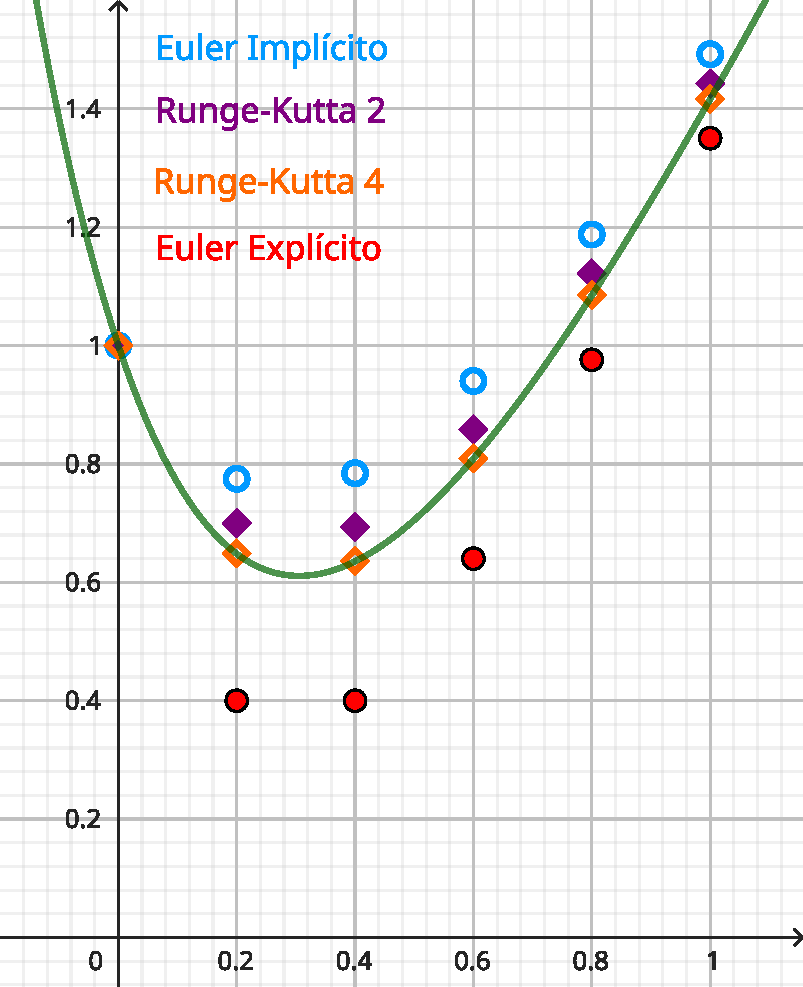
\includegraphics[width=0.4\textwidth]{img/edo-comparação.pdf}
\end{center}
\end{enumerate}
\end{document}
